214. \begin{figure}[ht!]
\center{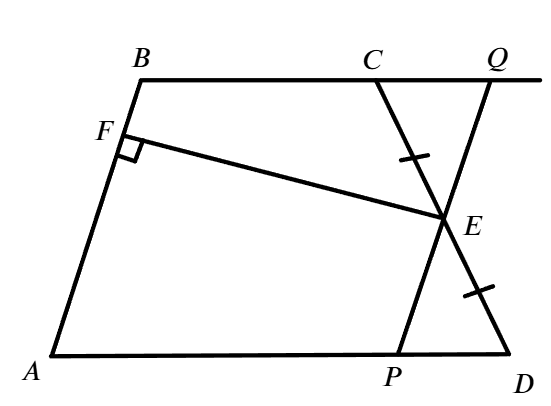
\includegraphics[scale=0.35]{g9-209.png}}
\end{figure}\\
Проведём через точку $E$ прямую, параллельную стороне $AB,$ пусть она пересекает сторону $AD$ в точке $P,$ а продолжение стороны $BC$ --- в точке $Q.$ Тогда четырёхугольник $ABQP$ является параллелограммом, а треугольники $PED$ и $QEC$ равны по стороне и двум прилежащим к ней углам ($DE=CE,$ углы $CEQ$ и $DEP$ вертикальные, а $ECQ$ и $EDP$ --- накрест лежащие). Поэтому их площади равны, и тогда $S_{ABCD}=S_{ABQP}=EF\cdot AB=4\cdot5=20.$
ewpage
oindent
